(by Vipin Singh)

This chapter presents an analysis of the team structure essential for executing the business model.
It outlines the various roles within the organization and their contributions towards achieving the business objectives.
The focus lies on understanding the division of responsibilities and the collaborative efforts necessary for the company's growth and success.
This examination is intended to provide a clear view of the organizational framework and its significance in the operational realization of the business strategy.

\p
Since the business idea will start in a small scale, the human resources need to be used as efficiently as possible.
With only five founder members, this requires that each members role is not just defined by their job title.
Instead each member will have to be able to adapt and contribute across various facets of the business.
Still the business should also be able to scale up and expand its operations as it grows.

\p
With this said lets analyze the team composition, that is focused to rapidly develop and launch the product.

%TODO: Maybe create the table inline?
\begin{figure}[H]
    \centering
    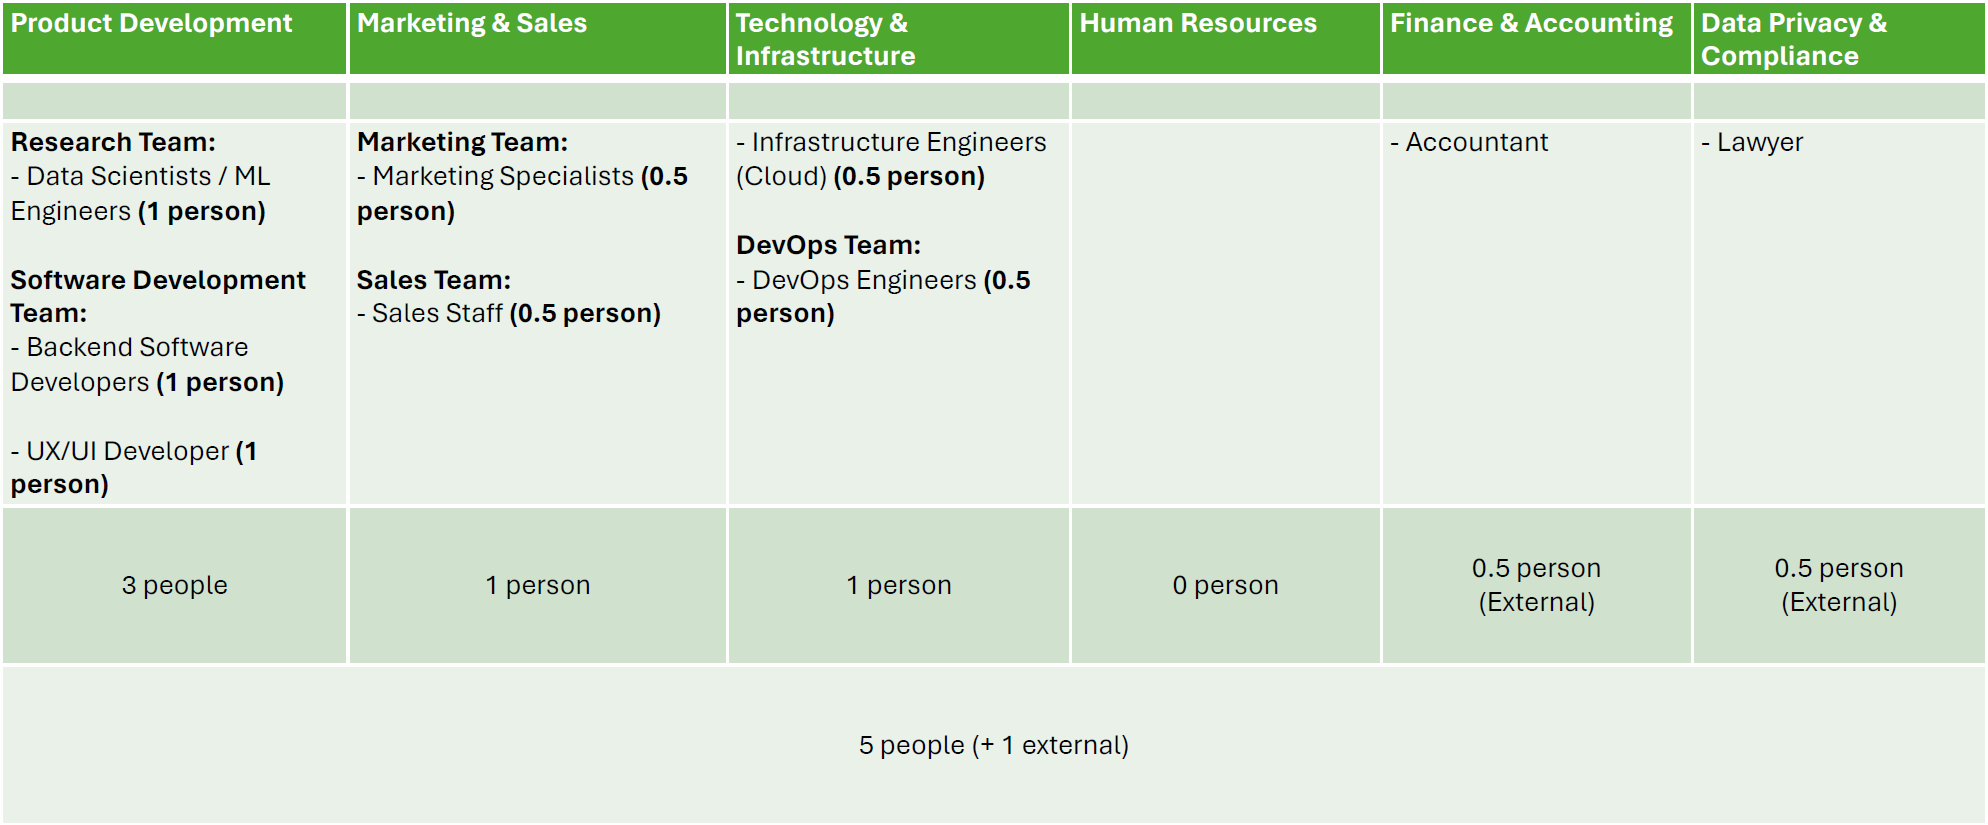
\includegraphics[width=\textwidth]{figures/team_comp_startup.png}
    \caption{Departments with team composition for a startup}
    \label{fig:team_comp_startup}
\end{figure}

%TODO: Maybe create the table inline?
\begin{figure}[H]
    \centering
    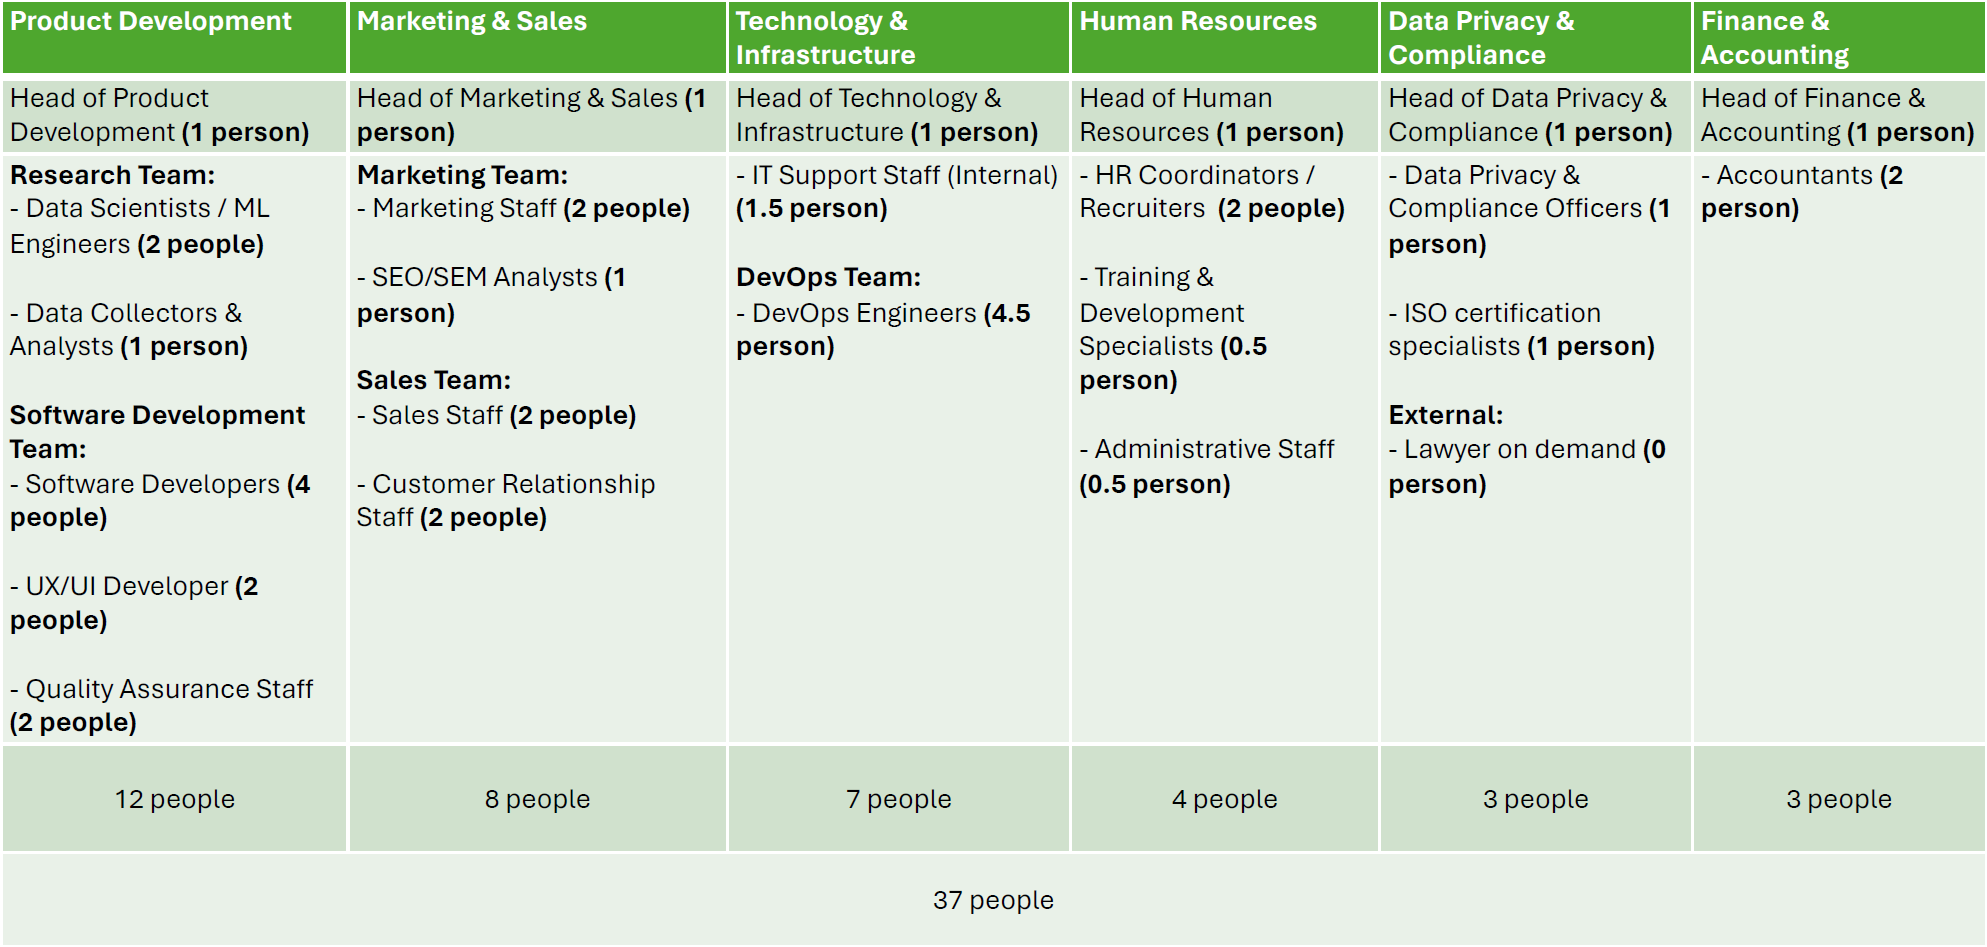
\includegraphics[width=\textwidth]{figures/team_comp_highscaled.png}
    \caption{Departments with team composition after the company has scaled up}
    \label{fig:team_comp_highscaled}
\end{figure}